\subsection{Configurazione} \label{configurazione}

		\subsubsection{Scopo del processo}

			Il processo di gestione della configurazione applica procedure tecniche ed amministrative
			lungo tutto il ciclo di vita del software. 
			Gli obiettivi di questo processo sono:

                \begin{itemize}
                    \item identificare e definire gli elementi software in un sistema;
                    \item controllare modifiche e rilasci degli elementi software;
                    \item registrare e riportare lo stato degli elementi software e delle richieste
                    di modifica;
                    \item garantire completezza, correttezza e coerenza degli elementi software;
                    \item controllare conservazione, gestione e consegna degli elementi software.
                \end{itemize}

        % modificato leggermente con "si utilizza" al posto di "si è utilizzato" perché stiamo normando non raccontando
	    \subsubsection{Processi di versionamento}

            Per il versionamento del software e della documentazione,
            si utilizza il software di controllo di versione \glossaryItem{Git}. In particolare il servizio \glossaryItem{GitHub}.

                \begin{figure}[htbp]
                    \centering
                    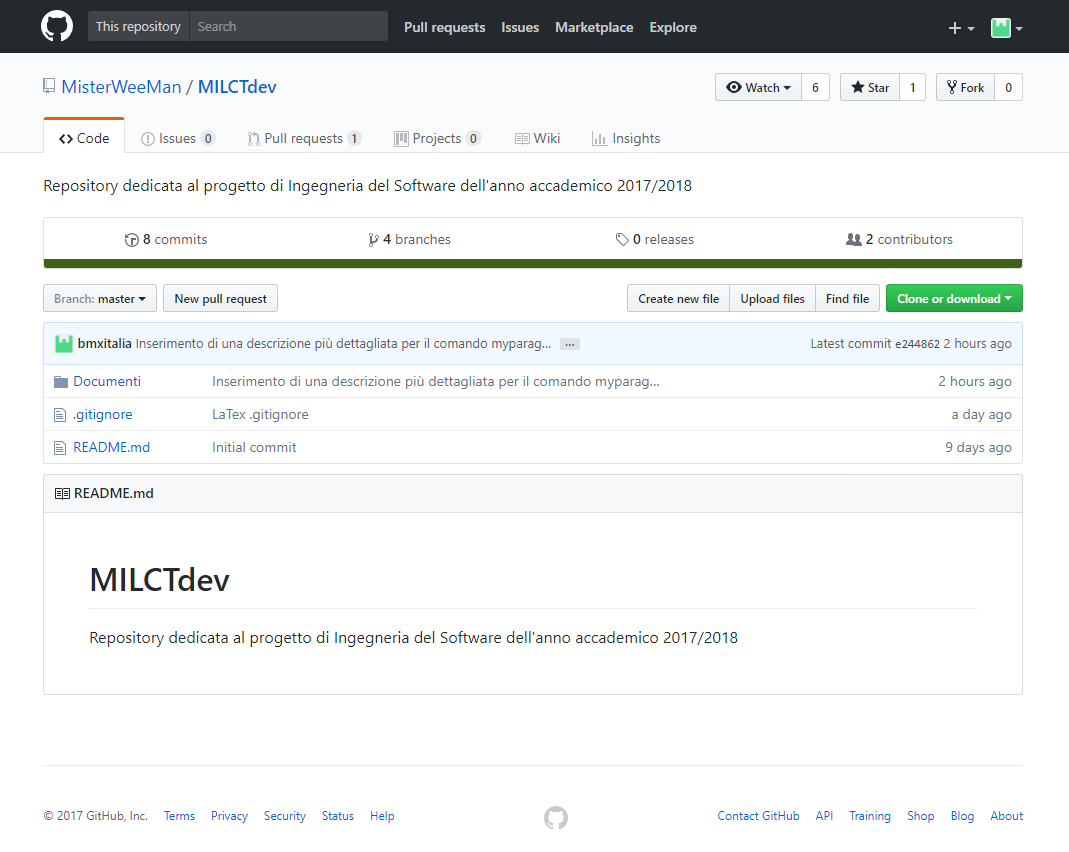
\includegraphics[height=9cm]{./img/gitHub.png}
                    \caption[GitHub]{GitHub: strumento  utilizzato dal gruppo per il controllo di versione}
                \end{figure}

            \myparagraph{Struttura della copia locale del repository}

                La copia locale della repository è composta da tre ``alberi" mantenuti da Git.
                Il primo è la directory di lavoro che contiene i files attuali su cui si sta lavorando.
                Il secondo è l'index (\glossaryItem{stage}) che fa da spazio di transito per i files.
                Per finire c'è l'\glossaryItem{head}, che punta all'ultimo \glossaryItem{commit} fatto.

                    \begin{figure}[htbp]
                        \centering
                        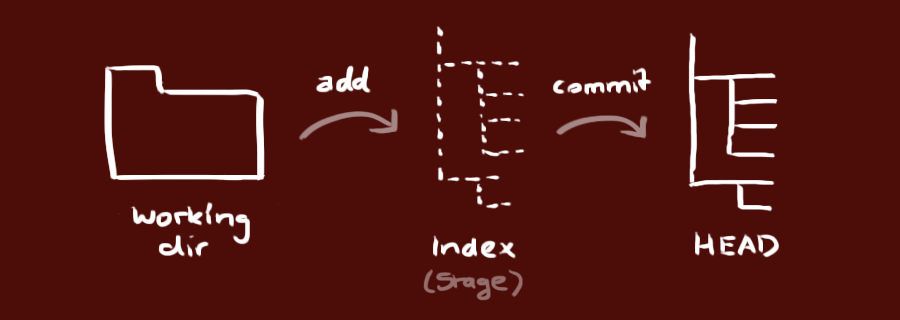
\includegraphics[scale=0.4]{./img/trees.png}
                        \caption[Struttura repository locale]{Struttura della repository locale, divisa nei tre alberi: working dir, stage e head}
                    \end{figure}

		    \myparagraph{Codici di versione della documentazione}\label{codici}

			    Come illustrato nella \S\ref{formatoFile}. il nome di
                un documento presenza il codice \_vX.Y.Z che rappresenta la versione del documento.
                Il significato delle lettere è il seguente:

                    \begin{itemize}
                        \item \textbf{Z}: è un numero che viene incrementato di uno ogni volta che viene
                        apportata una modifica al documento. Questo numero viene incrementato da colui che
                        ha apportato la modifica;
                        \item \textbf{Y}: è un numero che viene incrementato di uno ogni volta che il documento
                        è stato verificato da un Verificatore. È quindi compito del Verificatore incrementare
                        questo numero, nessun altro membro del team può farlo;
                        \item \textbf{X}: è un numero che viene incrementato di uno ogni volta che il documento
                        viene approvato dal Responsabile di Progetto per il rilascio. È compito del Responsabile di Progetto
                        incrementare questo numero. Ogni volta che un documento raggiunge l'approvazione può
                        essere generato il file pdf del documento.
                    \end{itemize}

                Ogni volta che un numero viene incrementato, tutti i numeri alla sua destra devono essere settati a zero.
